%!TEX root = ../../../main.tex
\section{Human Machine Interface} % (fold)
\label{sec:mr_human_machine_interface}

A Human Machine Interface (HMI) is an indispensable part of all complex robotic and automation systems. It not only makes it possible for the operators to gain manual control over specific subsystems or the whole system, but can provide feedback on its state and performance, and serve as a mean of intervention in emergency situations.

To reduce the risk of having communication failures rendering user interaction impossible, we have opted to pursue a redundant HMI solution, consisting of both a virtual and a physical User Interface introduced in the following sections.

	\subsection{Virtual UI} % (fold)
	\label{sub:mr_web}
	
	The virtual system is implemented following the Model-View-Controller architecture, where clients are connected to a central server unit. 
	
	\begin{figure}[H]
		\centering
	    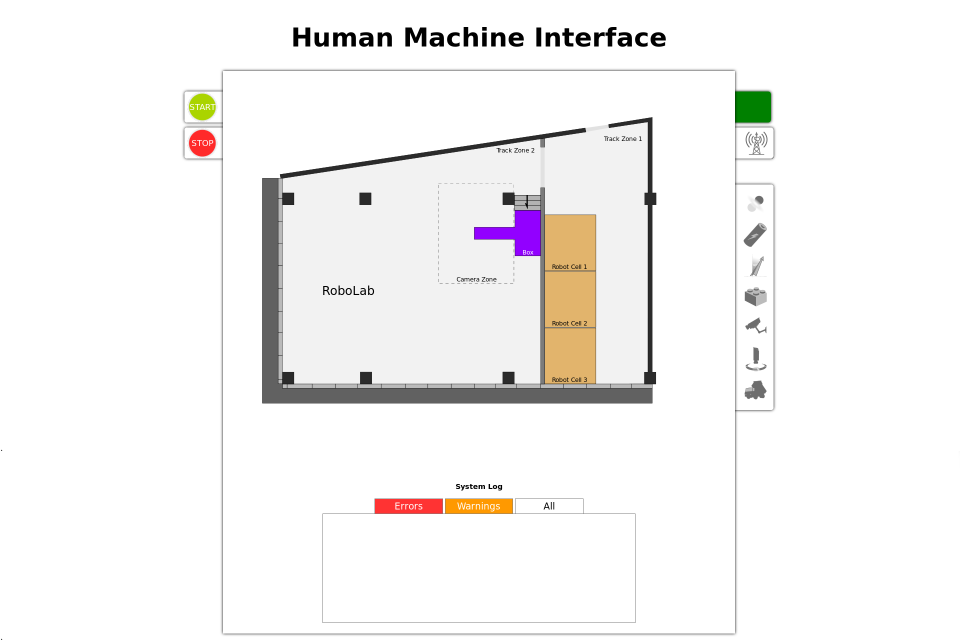
\includegraphics[width=0.95\textwidth]{mr_hmi_1}
	    \caption{Regular user interface for the mobile platform}
		\label{fig:mr_hmi_1}
	\end{figure}
	
	On the client side, a web application - written in HTML\cite{html} and formatted by CSS\cite{css} - is rendered through a web browser serving as the view. JavaScript\cite{javascript} modules are run in the background handling user interaction and the updating of the interface. The model used for communication is well defined through a protocol described in the appendix section \ref{"apx:com_prot"}. The UI is divided into two parts: a regular - see Figure \ref{fig:mr_hmi_1} - and an advanced interface - see Figure \ref{fig:mr_hmi_2}. This decision was motivated by the fact, that the information displayed on the UI, as well as the on, off and the emergency stop buttons can be useful even for those users who lack the inner understanding of the system. By separating the other functionality, such as the manual controls and the textual interfaces from the rest, we prevented any unintentional harm caused by the unskilled utilization of the HMI.
	
	On the server side, a proxy - written in Python\cite{python} - conveys the messages published by the ROS\cite{ros} components to the client, and vice versa. The client-server communication is based on WebSocket\cite{ws} technology - we are using the Autobahn|Python\cite{autobahn} - Twisted\cite{twisted} implementation -, which enables full duplex communication between the parties.
	
	The system is completely platform independent, requires no installation at the user end, and only a minimal set-up on the server side. This aspect of an industrial application is most desirable, since it leads to faster deployment times and minimized costs arising from dependency issues.
	
	\begin{figure}[H]
		\centering
		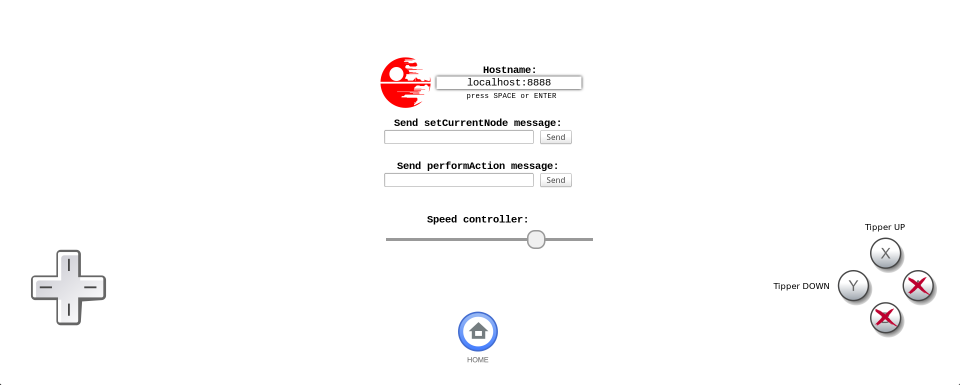
\includegraphics[width=0.95\textwidth]{mr_hmi_2}
		\caption{Advanced user interface for the mobile platform}
		\label{fig:mr_hmi_2}
	\end{figure}
	
	The virtual system has the following capabilities:
	
	\begin{itemize}
		\item Displaying of messages broadcast by various subsystems, with different views for the separate message types, namely: Errors, Warnings and all
		\item Possibility to change the operation mode of the mobile platform through user interaction
		\item Broadcast of an emergency signal
		\item Robot location and activity information display
		\item Provision of manual control of robot movement - with speed adjustment - and tipper states
		\item Provision of textual command interfaces
		\item Separation of normal and advanced features
		\item Automatic error handling in relation to connection malfunctioning 
	\end{itemize}

	% subsection web (end)

	\subsection{Physical UI} % (fold)
	\label{sub:mr_physical_devices}
	The user can control the mode of the robot with two buttons integrated in a button-board (see section \ref{sub:mr_buttons_board}).
	This board integrates two buttons: One for changing the mode of the robot to \emph{auto} and the other to \emph{idle}. These two modes are explained in section \ref{sec:mr_flow_control_overview}.

	At the same time, the board integrates a RGB led that change its color and the blink frequency to express different modes and actions.
	The different indications of the LED are shown in the appendix \ref{sec:buttons_board_s_led_meaning}.

	%\subsection{ROS Services} % (fold)
	%\label{sub:mr_ros_services}
	%Furthermore, the possibility of controlling the robot and knowing its states using ROS services, is given.
	%Due to the implementation of the code the project uses services intensively.
	%This allows to control the robot from the terminal and check the status by \emph{echoing} the publishers.
	% subsection ros_services (end)

% section human_machine_interface (end)